\section{The Cartan--Serre map} \label{s:comparison}

Let us consider, with their usual CW structures, the topological simplex $\gsimplex^n$ and the topological cube $\gcube^n$.
In \cite[p. 442]{serre1951homologie}, Serre described a quasi-isomorphism of coalgebras between the simplicial and cubical singular chains of a topological space.
It is given by precomposing with a canonical cellular map $\cs \colon \gcube^n \to \gsimplex^n$ also considered in \cite[p.199]{eilenberg1953acyclic} where it is attributed to Cartan.

The goal of this section is to deduce from a more general categorical statement that this comparison map between singular chains of a space is a quasi-isomorphism of $E_\infty$-coalgebras.

\subsection{Simplicial sets} \label{ss:simplicial sets}

We denote the \textit{simplex category} by $\simplex$, the category $\Fun(\simplex^\op, \Set)$ of \textit{simplicial sets} by $\sSet$, and the representable simplicial set $\yoneda \big( [n] \big)$ by $\simplex^n$.
As usual, we denote an element in $\simplex^n_m$ by a non-decreasing tuple $[v_0, \dots, v_m]$ with $v_i \in \{0, \dots, n\}$.
The \textit{Cartesian product} of simplicial sets is defined by the product of functors.
The \textit{simplicial $n$-cube} $\scube{n}$ is the $n^\th$-fold Cartesian product of $\simplex^1$ with itself.

We will use the following model of the topological $n$-simplex:
\[
\gsimplex^n = \big\{ (y_1, \dots, y_n) \in \gcube^n \mid i \leq j \Rightarrow y_i \geq y_j \big\},
\]
whose cell structure associates $[v_0, \dots, v_m]$ with the subset
\begin{equation} \label{e:cell structure of gsimplex}
	\Big\{ \big( \underbrace{1, \dots, 1}_{v_0}, \underbrace{y_1, \dots y_1}_{v_1-v_0}, \dots, \underbrace{y_m, \dots y_m}_{v_m-v_{m-1}}, \underbrace{0, \dots, 0}_{n-v_m} \big) \mid y_1 \geq \dots \geq y_m \Big\}.
\end{equation}
The spaces $\gsimplex^n$ define a functor $\simplex \to \CW$ with
\begin{align*}
	\sigma_i(x_1, \dots, x_n) &= (x_1, \dots, \widehat x_i, \dots, x_n) \\
	\delta_0(x_1, \dots, x_n) &= (1, x_1, \dots, x_n), \\
	\delta_i(x_1, \dots, x_n) &= (x_1, \dots, x_i, x_i, \dots, x_n), \\
	\delta_n(x_1, \dots, x_n) &= (x_1, \dots, x_n, 0).
\end{align*}
Its Yoneda extension is the \textit{geometric realization} functor.
It has a right adjoint $\sSing \colon \Top \to \sSet$ referred to as the \textit{simplicial singular complex} satisfying
\[
\sSing(\fZ)_n = \Top(\gsimplex^n, \fZ)
\]
for any topological space $\fZ$.

The functor of (\textit{normalized}) \textit{chains} $\schains \colon \sSet \to \Ch$ is the composition of the geometric realization functor and that of cellular chains.
We denote the composition $\schains \circ \sSing$ by $\sSchains$ and omit the superscript $\simplex$ if no confusion may result from doing so.
For any $n \in \N$, the \textit{Alexander--Whitney coalgebra structure} on $\chains(\simplex^n)$ is given by
\[
\Delta \big( [v_0, \dots, v_m] \big) = \sum_{i=0}^m [v_0, \dots, v_i] \ot [v_i, \dots, v_m],
\]
and
\[
\epsilon \big( [v_0, \dots, v_m] \big) =
\begin{cases}
	1 & \text{ if } m = 0, \\ 0 & \text{ if } m>0.
\end{cases}
\]
The degree 1 product $\ast \colon \chains(\simplex^n)^{\ot 2} \to \chains(\simplex^n)$ is defined by
\begin{align*}
	\begin{autobreak}
		\left[v_0, \dots, v_p \right] \ast
		\left[v_{p+1}, \dots, v_m\right] =
		{\begin{cases}
			(-1)^{p+|\sigma|} \left[v_{\sigma(0)}, \dots, v_{\sigma(m)}\right] &
			\text{ if } v_i \neq v_j \text{ for } i \neq j, \\
			0 & \text{ if not},
		\end{cases}}
	\end{autobreak}
\end{align*}
where $\sigma$ is the permutation that orders the totally ordered set of vertices and $(-1)^{|\sigma|}$ is its sign.
As shown in \cite[Theorem 4.2]{medina2020prop1} the assignment
\[
\counit \mapsto \epsilon, \quad \coproduct \mapsto \Delta, \quad \product \mapsto \ast,
\]
defines a natural $\M$-bialgebra on the chains of representable simplicial sets, and, by forgetting structure, also a natural $\UM$-coalgebra.
For any simplicial set, a natural $\UM$-coalgebra structure on its chains is defined by a Yoneda extension.

\subsection{The Eilenberg--Zilber maps} \label{ss:ez}

For any permutation $\sigma \in \sym_n$ let
\[
\gi_\sigma \colon \gsimplex^n \to \gcube^n
\]
be the inclusion defined by $(x_1, \dots, x_n) \mapsto (x_{\sigma(1)}, \dots, x_{\sigma(n)})$.
If $e$ is the identity permutation, we denote $\mathfrak{i}_{e}$ simply as $\mathfrak{i}$.
%and notice that it satisfies $\cs \circ\, \mathfrak{i} = \id_{\gsimplex^n}$.
The maps $\set{\mathfrak{i}_\sigma}_{\sigma \in \sym_n}$ define a subdivision of $\gcube^n$ making it isomorphic to $\bars[\big]{\scube{n}}$ in $\CW$.
Using this identification, the identity map induces a cellular map
\[
\ez \colon \gcube^n \to \bars[\big]{\scube{n}}.
\]
We denote the induced chain map by
\[
\EZ \colon \chains(\cube^n) \to \chains\big(\scube{n}\big).
\]
For any topological space $\fZ$, the cubical map
\[
\cubify\sSing(\fZ) \to \cSing(\fZ)
\]
is defined, using the adjunction isomorphism
\[
\sSet\big(\scube{n}, \sSing(\fZ)\big) \cong
\Top\big(\bars{\scube{n}}, \fZ\big),
\]
by the assignment
\[
\big( \bars{\scube{n}} \xra{f} \fZ \big) \mapsto
\big( \gcube^n \xra{\ez} \bars{\scube{n}} \xra{f} \fZ \big).
\]
We denote the induced chain map by
\[
\EZ_{\Schains(\fZ)} \colon
\cchains\!\big(\cubify\sSing(\fZ)\big) \to \cSchains(\fZ).
\]
%Please note that $\nu_\fZ$ is a cubical map given the naturality of $\ez$.

%% POSSIBLE REMARK
%Using the isomorphism $\chains(\cube^n) \cong \chains(\cube^1)^{\ot n} \cong \chains(\simplex^1)^{\ot n}$, this map agrees with the usual Eilenberg--Zilber maps $\chains(\simplex^1)^{\ot n} \to \chains \big( \scube{n} \big)$.

%% EXPLORE LATER
%For any topological space $\fZ$ we have a quasi-isomorphism
%\begin{equation} \label{e:ezz}
%	\begin{tikzcd} [column sep=small, row sep=0]
%		\EZ_{\Schains(\fZ)} \colon &[-20pt] \cSchains(\fZ) \arrow[r] & \sSchains (\fZ) \\
%		& (\gcube^n \to \fZ) \arrow[r, mapsto] &
%		\sum\limits_{\mathclap{\sigma \in \sym_n}} \sign(\sigma) \big( \gsimplex^n \xra{\gi_\sigma} \gcube^n \to \fZ \big).
%	\end{tikzcd}
%\end{equation}

\subsection{The Cartan--Serre maps}

The cellular map
\[
\cs \colon \gcube^n \to \gsimplex^n
\]
is defined by
\[
\cs(x_1, \dots, x_n) =
(x_1,\ x_1 x_2, \, \dots \, , \ x_1 x_2 \dotsm x_n).
\]
We denote its induced chain map by
\[
\CS \colon \chains(\cube^n) \to \chains(\simplex^n).
\]
%by applying the functor of cellular chains to $\cs \colon \gcube^n \to \gsimplex^n$.
The chain map
\[
\CS_{\Schains(\fZ)} \colon \sSchains(\fZ) \to \cSchains(\fZ)
\]
between the singular chain complexes of a topological space $\fZ$ is defined by
\[
\CS_{\Schains(\fZ)} (\gsimplex^n \to \fZ) =
(\gcube^n \xra{\cs} \gsimplex^n \to \fZ).
\]
%\[
%\begin{tikzcd} [column sep=small, row sep=0]
%	\CS_{\Schains(\fZ)} \colon &[-25] \sSchains(\fZ) \arrow[r] & \cSchains (\fZ) \\ &
%	(\gsimplex^n \to \fZ) \arrow[r, mapsto] & (\gcube^n \xra{\cs} \gsimplex^n \to \fZ).
%\end{tikzcd}
%\]

These maps were considered in \cite[p. 442]{serre1951homologie} where it was stated that $\CS_{\Schains(\fZ)}$ is a natural quasi-isomorphisms of coalgebras.
We will prove this in \cref{ss:e-infty preservation} showing in fact that it is a quasi-isomorphism of $E_\infty$-coalgebras.

\subsection{No-go results}

Since $\CS$ is shown to be a coalgebra map in \cref{l:cs coalgebra map} and $\EZ$ is well known to be one, one may hope for higher structures to be preserved by these maps.
We now provide some examples constraining the scope of these expectations.

\begin{example*}
	We will show that $\EZ$ does not preserve $\UM$-structures.
	More specifically, that in general
	\[
	\EZ^{\ot 2} \circ \, \Delta_1 \neq \Delta_1 \circ \EZ
	\]
	where
	\[
	\Delta_1 = (\ast \ot \id) \circ (\id \ot (12) \Delta) \circ \Delta
	\]
	is the cup-1 coproduct presented in \cref{e:closed cup-i}.
	Up to signs, on one hand we have
	\begin{align*}
		\begin{autobreak}
			\Delta_1 \big( [01] [01] \big)
			= [01][01] \ot [1][01]
			\ +\ [01][1] \ot [01][01]
			\ +\ [0][01] \ot [01][01]
			\ +\ [01][01] \ot [01][0].
		\end{autobreak}
	\end{align*}
%	\begin{multline*}
%		\Delta_1 \big( [01] [01] \big) = \\
%		[01][01] \ot [1][01] + [01][1] \ot [01][01] + [0][01] \ot [01][01] + [01][01] \ot [01][0].
%	\end{multline*}
	Therefore,
	\begin{align*}
		\begin{autobreak}
			\EZ^{\ot 2} \circ \, \Delta_1 \big( [01][01] \big)
			= \big( 011\times001 + 001\times011 \big) \ot 11 \times 01
			\ +\ 01\times11 \ot \big( 011\times001+ 001\times011 \big)
			\ +\ 00\times01 \ot \big( 011\times001 + 001\times011 \big)
			\ +\ \big( 011\times001 + 001\times011 \big) \ot 01\times00.
		\end{autobreak}
	\end{align*}
%	\begin{multline*}
%		\EZ^{\ot 2} \circ \, \Delta_1 \big( [01][01] \big) =
%		\big( 011\times001 + 001\times011 \big) \ot 11 \times 01 \ +\
%		01\times11 \ot \big( 011\times001 + 001\times011 \big) \ +\ \\
%		00\times01 \ot \big( 011\times001 + 001\times011 \big) \ +\
%		\big( 011\times001 + 001\times011 \big) \ot 01\times00.
%	\end{multline*}
	On the other hand, we have
	\[
	\Delta_1 [0,1,2] = [0,1,2] \ot [0,1] + [0,2] \ot [0,1,2] + [0,1,2] \ot [1,2].
	\]
	Therefore,
%	\begin{multline*}
%		\Delta_1 \circ \EZ \big( [01] [01] \big) = \Delta_1 \big( 011\times001 + 001\times011 \big) = \\
%		011\times001 \ot 01\times00 \ + \
%		01\times01 \ot 011\times001 \ + \
%		011\times001 \ot 11\times01 \ + \ \\
%		001\times011 \ot 00\times01 \ + \
%		01\times01 \ot 001\times011 \ + \
%		001\times011 \ot 01\times11.
%	\end{multline*}
	\begin{align*}
		\begin{autobreak}
			\Delta_1 \circ \EZ \big( [01] [01] \big)
			= \Delta_1 \big( 011\times001 + 001\times011 \big)
			= 011\times001 \ot 01\times00
			\ + \ 01\times01 \ot 011\times001
			\ + \ 011\times001 \ot 11\times01
			\ + \ 001\times011 \ot 00\times01
			\ + \ 01\times01 \ot 001\times011
			\ + \ 001\times011 \ot 01\times11.
		\end{autobreak}
	\end{align*}
	We conclude that
	\[
	\EZ^{\ot 2} \circ \, \Delta_1 \big( [01][01] \big) \neq \Delta_1 \circ \EZ \big( [01] [01] \big)
	\]
	since, for example, the basis element $01\times11 \ot 011\times001$ appears in the left sum but not in the right one.
\end{example*}

\begin{example*}
	We will show that the Cartan--Serre map does not preserve $\M$-structures.
	More specifically, that in general
	\[
	\CS(x \ast y) \neq \CS(x) \ast \CS(y).
	\]
	Consider $x = [1][1]$ and $y = [0][01]$.
	On one hand we have that
	\[
	\CS \big( [1][1] \big) \ast \CS \big( [0][01] \big) = 0
	\]
	since $\CS \big( [0][01] \big) = 0$.
	On the other hand we have, up to a signs, that
	\[
	\CS \Big( ([1][1]) \ast ([0][01]) \Big) =
	\CS \Big( [01][01] \Big) = [012],
	\]
	which establishes the claim.
\end{example*}

The reason for this incompatibility is that $\ast$ in the simplicial context is commutative, which is not the case in the cubical one.

\begin{example*}
	We will show that the Cartan--Serre map does not preserve $\UM$-structures.
	More specifically, that in general
	\[
	\CS \circ\, \widetilde\Delta_1 \neq
	\widetilde\Delta \circ \CS
	\]
	where
	\[
	\widetilde\Delta_1 =
	(\ast \ot \id) \circ (12) (\id \ot (12) \Delta) \circ \Delta.
	\]
	On one hand we have that
	\[
	\CS\Big( \widetilde\Delta_1 \big( [01][01] \big) \Big) =
	T \Delta_1 \big( [012] \big),
	\]
	and on the other that
	\[
	\widetilde\Delta_1 \circ \CS \big( [01][01] \big) =
	\Delta_1 \big( [012] \big),
	\]
	which establishes the claim.
\end{example*}

In \cref{ss:e-infty preservation} we will show that $\CS$ is a morphism of $E_\infty$-coalgebras.
To do so we now introduce an $E_\infty$-suboperad of $\UM$ where the incompatibility resulting from the lack of commutativity of $\ast$ in the cubical context is dealt with.

\subsection{Shuffle graphs} \label{ss:shuffle graphs}

Consider $k = k_1+\dots+k_r$.
A $(k_1,\dots,k_r)$-shuffle $\sigma$ is a permutation in $\sym_{k}$ satisfying
\begin{align*}
	&\sigma(1) < \dots < \sigma(k_1), \\
	&\sigma(k_1+1) < \dots < \sigma(k_1+k_2), \\
	&\qquad \vdots \\
	&\sigma(k-k_r+1) < \dots < \sigma(k).
\end{align*}
The (\textit{left comb}) \textit{shuffle graph} associated to such $\sigma$ is the $(1,k)$-graph
\[
\boxed{\documentclass{standalone}
\usepackage{tikz}
\usepackage{amsmath}

\begin{document}
	\begin{tikzpicture}[scale=1.5]
		\coordinate (o) at (0,0);
		\draw (o)--(0,-.4) node[below, scale=.7]{$1$};
		\draw (o)--(-.6,.6) node[above, scale=.7]{$1$\hspace{0pt}};
		\draw (-.4,.4)--(-.2,.6) node[above, scale=.7]{$2$\hspace{0pt}};
		\draw (o)--(.6,.6) node[above, scale=.7]{\hspace{0pt} $k_1$};
		\node[scale=.7] at (.1,.5){...};
		\node[scale=.7] at (.2,.72){...};
		\node at (1.1,0){$\dots$};
	\end{tikzpicture}
	\hspace*{-16pt}
	\begin{tikzpicture}[scale=1.5]
		\coordinate (o) at (0,0);
		\draw (o)--(0,-.4) node[below, scale=.7]{$r$};
		\draw (o)--(-.6,.6) node[above, scale=.7]{$k-k_r+1$\hspace*{11pt}};
		\draw (-.15,.15)--(.3,.6) node[above, scale=.7]{$k-1$\hspace*{1pt}};
		\draw (o)--(.6,.6) node[above, scale=.7]{\hspace*{5pt} $k$};
		\node[scale=.7] at (-.15,.5){...};
		\node[scale=.7] at (-.1,.74){...};
		\node at (1,.05){$\circ$};
	\end{tikzpicture}
	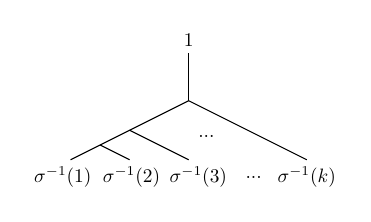
\begin{tikzpicture}[scale=1.5]
		\coordinate (o) at (0,0);
		\draw (o)--(0,.4) node[scale=.7, above]{$1$};
		\draw (o)--(-1,-.5) node[scale=.7, below]{$\sigma^{-1}(1)$\hspace*{8pt}};
		\draw (-.75,-.375)--(-.5,-.5) node[scale=.7, below]{\hspace*{2pt}$\sigma^{-1}(2)$};
		\draw (-.5,-.25)--(0,-.5) node[scale=.7, below]{\hspace*{10pt}$\sigma^{-1}(3)$};
		\draw (o)--(1,-.5) node[scale=.7, below]{$\sigma^{-1}(k)$};
		\node[scale=.7] at (.15,-.3){...};
		\node[scale=.7] at (.55,-.65){...};
	\end{tikzpicture}
\end{document}}
\]
presented as a composition of (left comb) self-graftings of the generators $\product$ and $\coproduct$.
With the notation introduced in \cref{e:iterated comb}, the $\UM$-coalgebra sends the shuffle graph associated to $\sigma$ to
\[
(\ast^{k_1} \ot \dotsb \ot \ast^{k_r}) \circ \sigma^{-1} \Delta^{k-1}.
\]

\begin{example*}
	All the graphs in \cref{f:cup-i} are shuffle graphs.
	In fact, all the cup-$i$ coproducts presented in \cref{e:closed cup-i} are induced from shuffle graphs, whereas
	\begin{align*}
		\widetilde\Delta_1 &=
		(\ast \ot \id) \circ (12) (\id \ot (12) \Delta) \circ \Delta \\ &=
		(\ast \ot \id) \circ (123) \Delta^2,
	\end{align*}
	used in the previous section to probe the limits of the structure preserving properties of $\CS$, is not.
\end{example*}

The operad $\UMsh$ is defined as the suboperad of $\UM$ (freely) generated by shuffle graphs.
Explicitly, any element in $\UMsh(r)$ is represented by a linear combination of $(1,r)$-graphs obtained by grafting these.
The same proof used in \cite[p.5]{medina2020prop1} to show that $\UM$ is an $E_\infty$-operad can be used to prove the same for $\UMsh$.

\subsection{$E_\infty$-coalgebra preservation} \label{ss:e-infty preservation}

We devote this subsection to the proof of the following key result.

\begin{theorem} \label{t:main local}
	The chain map $\CS \colon \chains(\cube^n) \to \chains(\simplex^n)$ is a quasi-isomorphism of $\UMsh$-coalgebras.
\end{theorem}

We start by stating an alternative description of the $\CS$ map.

\begin{lemma} \label{l:cs explicit}
	Let $x = x_1 \ot \cdots \ot x_n \in \chains(\cube^n)_m$ be a basis element with $x_{q_i} = [0,1]$ for all $\{q_1 < \dots < q_m\}$.
	If there is $x_\ell = [0]$ with $\ell < q_m$ then $\CS(x) = 0$, otherwise
	\[
	\CS(x) = \big[ q_1-1, \ \dots \, , \ q_m-1, \ p(x)-1 \big]
	\]
	where $p(x) = \min \set[\big]{\ell \mid x_\ell = [0]}$ or $p(x) = n+1$ if this set is empty.
\end{lemma}

\begin{proof}
	This can be directly verified using the cell structure of $\gsimplex^n$ described in \cref{e:cell structure of gsimplex}.
%	the fact that the image of $\cs \circ \, \delta^0_\ell \colon \gcube^{n-1} \to \gsimplex^n$ for $\ell \in \set{1,\dots,n-1}$ is in a lower dimensional skeleton of $\gsimplex^n$, and the identities
%	\[
%	\cs \circ \, \delta_\ell^1 = \delta_{i-1} \circ \cs,
%	\qquad
%	\cs \circ \, \delta_n^0 = \delta_n \circ \cs,
%	\]
%	for $\ell \in \set{1, \dots, n}$.
\end{proof}

\begin{lemma} \label{l:cs coalgebra map}
	The chain map $\CS \colon \chains(\cube^n) \to \chains(\simplex^n)$ is a quasi-isomorphism of coalgebras.
\end{lemma}

\begin{proof}
	The chain map $\CS$ is a quasi-isomorphism compatible with the counit since it is induced from a cellular map between contractible spaces.
	We need to show it preserves coproducts.
	By naturality it suffices to verify this on $[0,1]^{\ot n}$.
	Recall from \cref{l:coproduct description} that
	\[
	\Delta \big( [0,1]^{\ot n} \big) =
	\sum_{\lambda \in \Lambda} (-1)^{\ind \lambda} \
	\Big(x_1^{(\lambda)} \ot \cdots \ot x_n^{(\lambda)}\Big) \ot
	\Big(y_1^{(\lambda)} \ot \cdots \ot y_n^{(\lambda)}\Big),
	\]
	where the sum is over all choices for each $i \in \{1,\dots,n\}$ of
	\begin{align*}
		x_i^{(\lambda)} &= [0,1],&&\text{or} & x_i^{(\lambda)} &= [0], \\
		y_i^{(\lambda)} &= [1],  && & y_i^{(\lambda)} &= [0,1].
	\end{align*}
	By \cref{l:cs explicit}, the summands above not sent to $0$ by $\CS \ot \CS$ are those basis elements for which $x_i^{(\lambda)} = [0]$ implies $x_j^{(\lambda)} = [0]$ for all $i < j$.
	For any one such summand, its sign is positive and its image by $\CS \ot \CS$ is $[0, \dots, k] \ot [k, \dots, n]$ where $k+1 = \min\set[\big]{i \mid x_i^{(\lambda)} = [0]}$ or $k = n$ if this set is empty.
	The summands $[0, \dots, k] \ot [k,\dots,n]$ are precisely those appearing when applying the Alexander--Whitney coproduct to $\CS \big([0,1]^{\ot n}\big) = [0,\dots,n]$.
	This concludes the proof.
\end{proof}

We will consider the basis of $\chains(\cube^n)$ as a poset with
\[
(x_1 \ot \cdots \ot x_n) \leq (y_1 \ot \cdots \ot y_n)
\]
if and only if $x_\ell \leq y_\ell$ for each $\ell \in \{1, \dots, n\}$ with respect to
\[
[0] < [0,1] < [1].
\]
As we prove next, an example of ordered elements are the tensor factors of each summand in the iterated Serre diagonal.

\begin{lemma} \label{l:order iterated coproduct}
	Writing
	\[
	\Delta^{k-1} \big([0,1]^{\ot n}\big) =
	\sum \pm \ x^{(1)} \ot \cdots \ot x^{(k)}
	\]
	with each $x^{(\ell)}$ a basis element of $\chains(\cube^n)$, we have
	\[
	x^{(1)} \leq \cdots \leq x^{(k)}
	\]
	for every summand.
\end{lemma}

\begin{proof}
%	For $k = 2$, recall from \cref{l:coproduct description} that
%	\[
%	\Delta \big( [0,1]^{\ot n} \big) =
%	\sum_{\lambda \in \Lambda} (-1)^{\ind \lambda} \
%	\Big(x_1^{(\lambda)} \ot \cdots \ot x_n^{(\lambda)}\Big) \ot
%	\Big(y_1^{(\lambda)} \ot \cdots \ot y_n^{(\lambda)}\Big),
%	\]
%	where the sum is over all choices for each $i \in \{1,\dots,n\}$ of
%	\begin{align*}
%		x_i^{(\lambda)} &= [0,1],&&\text{or} & x_i^{(\lambda)} &= [0], \\
%		y_i^{(\lambda)} &= [1],  && & y_i^{(\lambda)} &= [0,1].
%	\end{align*}
%
%
%	and any $\ell \in \{1, \dots, n\}$ we have that
%	\begin{align*}
%		x^{(1)}_\ell = [0]  & \iff x^{(2)}_\ell = [0,1], \\
%		x^{(1)}_\ell = [0,1] & \iff x^{(2)}_\ell = [1],
%	\end{align*}
%	and that neither $x^{(1)}_\ell = [1]$ or $x^{(2)}_\ell = [0]$ can occur, hence $x^{(1)} \leq x^{(2)}$.
%	The claim for $k > 2$ follows from a straightforward induction argument.
	This can be proven using a straightforward induction argument whose base case follows from inspecting \cref{l:coproduct description}.
\end{proof}

\begin{lemma}
	Let $x$, $y$ and $z$ be basis elements of $\chains(\cube^n)$.
	If both $x \leq z$ and $y \leq z$ then either $(x \ast y) = 0$ or every summand in $(x \ast y)$ is $\leq z$.
\end{lemma}

\begin{proof}
	Recall that
	\begin{multline*}
		(x_1 \ot \cdots \ot x_n) \ast (y_1 \ot \cdots \ot y_n)
		=
		(-1)^{|x|} \sum_{\ell=1}^n x_{<\ell}\, \epsilon(y_{<\ell}) \ot x_\ell \ast y_\ell \ot \epsilon(x_{>\ell}) \, y_{>\ell}.
	\end{multline*}
	By assumption $x_{<\ell} \leq z_{<\ell}$ and $y_{>\ell} \leq z_{>\ell}$ for every $\ell \in \{1, \dots, n\}$.
	If $x_\ell \ast y_\ell \neq 0$ then $x_\ell \ast y_\ell = [0,1]$ and either $x_\ell = [1]$ or $y_\ell = [1]$ which implies $z_\ell = [1]$ as well, so $x_\ell \ast y_\ell \leq z_\ell$.
\end{proof}

\begin{lemma}
	If $x$ and $y$ are basis elements of $\chains(\cube^n)$ satisfying $x \leq y$ then
	\begin{equation} \label{e:cs collapse as algebra map}
		\CS(x \ast y) = \CS(x) \ast \CS(y).
	\end{equation}
\end{lemma}

\begin{proof}
	We present this proof in the form of three claims.
	We use \cref{l:cs explicit}, the assumption $x \leq y$, and the fact that the join of basis elements in $\chains(\simplex^n)$ sharing a vertex is $0$ without explicit mention.

	\medskip\noindent \textit{Claim 1}.
	If $\CS(x) = 0$ or $\CS(y) = 0$ then for every $i \in \{1, \dots, n\}$
	\begin{equation} \label{e:zero for join}
		\CS \big( x_{<i}\, \epsilon(y_{<i}) \ot x_i \ast y_i \ot \epsilon(x_{>i}) \, y_{>i} \big) = 0.
	\end{equation}
	Assume $\CS(x) = 0$, that is, there exists a pair $p < q$ such that $x_p = [0]$ and $x_q = [0,1]$, then \eqref{e:zero for join} holds since:
	\begin{enumerate}
		\item If $i > q$, then $x_p$ and $x_q$ are part of $x_{<i}$.
		\item If $i = q$, then $x_q \ast y_q = 0$ for any $y_q$.
		\item If $i < q$, then $\epsilon(x_{>i}) = 0$.
	\end{enumerate}
	Similarly, if there is a pair $p < q$ such that $y_p = [0]$ and $y_q = [0,1]$, then \eqref{e:zero for join} holds since:
	\begin{enumerate}
		\item If $i < p$, then $y_p$ and $y_q$ are part of $y_{>i}$.
		\item If $i = p$, then $x_i = [0]$ and $x_i \ast y_i = 0$.
		\item If $i > p$, then either $x_i \ast y_i = 0$ or $x_i \ast y_i = [0,1]$ and $x_p = [0]$.
	\end{enumerate}
	This proves the first claim and identity \eqref{e:cs collapse as algebra map} under its hypothesis.

	\medskip\noindent \textit{Claim 2}.
	If $\CS(x) \neq 0$ and $\CS(y) \neq 0$ then
	\[
	\CS(x \ast y) =
	\CS \big( x_{<p_x} \epsilon(y_{<p_x}) \ot \, x_{p_x} \! \ast y_{p_x} \ot \epsilon(x_{>p_x}) \, y_{>p_x} \big)
	\]
	if $p_x = \min \big\{ i \mid x_i = [0] \big\}$ is well-defined and $x \ast y = 0$ if not.

	\medskip Assume $p_x$ is not well-defined, i.e., $x_i \neq [0]$ for all $i \in \{1, \dots, n\}$.
	Given that $x \leq y$ we have that $[0] < x_i$ implies $x_i \ast y_i = 0$, and the claim follows in this case.

	Assume $p_x$ is well-defined.
	We will show that for all $i \in \{1,\dots,n\}$ with the possible exception of $i = p_x$ we have
	\begin{equation} \label{e:case main lemma third claim}
		\CS \big( x_{<i} \, \epsilon(y_{<i}) \ot \, x_{i} \! \ast y_{i} \ot \epsilon(x_{>i}) \, y_{>i} \big) = 0
	\end{equation}
	This follows from:
	\begin{enumerate}
		\item If $i < p_x$ and $x_i = [1]$ then $y_i = [1]$ and $x_i \ast y_i = 0$.
		\item If $i < p_x$ and $x_i = [0,1]$ then $x_i \ast y_i = 0$ for any $y_i$.
		\item If $i > p_x$ then \cref{l:cs explicit} implies the claim since $x_{p_x} = [0]$ and $x_i \ast y_i \neq 0$ iff $x_i \ast y_i = [0,1]$.
	\end{enumerate}

	\noindent \textit{Claim 3}.
	If $\CS(x) \neq 0$ and $\CS(y) \neq 0$ then \eqref{e:cs collapse as algebra map} holds.

	\medskip Let us assume that $\big\{ i \mid x_i = [0] \big\}$ is empty, which implies the analogous statement for $y$ since $x \leq y$.
	Since neither of $x$ nor $y$ have a factor $[0]$ in them, \cref{l:cs explicit} implies that the vertex $[n]$ is in both $\CS(x)$ and $\CS(y)$, which implies $\CS(x) \ast \CS(y) = 0$ as claimed.

	Assume now that $p_x = \big\{ i \mid x_i = [0] \big\}$ is well defined, and let $\{q_1 < \dots < q_m\}$ with $x_{q_i} = [0,1]$ for $i \in \{1,\dots,m\}$.
	Since $\CS(x) \neq 0$ \cref{l:cs explicit} implies that $p_x > q_m$, so $\epsilon(x_{>p_x}) = 1$ and Claim 2 implies
	\[
	\CS(x \ast y) =
	\CS \big( x_{<p_x} \epsilon(y_{<p_x}) \ot \, x_{p_x} \! \ast y_{p_x} \ot y_{>p_x} \big).
	\]
	We have the following cases:
	\begin{enumerate}
		\item If $\epsilon(y_{<p_x}) = 0$ then there is $q_i$ such that $y_{q_i} = [0,1]$ so $[q_i-1]$ is in both $\CS(x)$ and $\CS(y)$.
		\item If $\epsilon(y_{p_x}) \neq 0$ and $y_{p_x} \in \{[0], [0,1]\}$ then $x_{p_x} \ast y_{p_x} = 0$ and $[p_x-1]$ is in both $\CS(x)$ and $\CS(y)$.
		\item If $\epsilon(y_{p_x}) \neq 0$ and $y_{p_x} = [1]$ let $\{\ell_1 < \dots < \ell_k\}$ be such that $y_{\ell_j} = [0,1]$ and let $p_y > \ell_k$ be either $n+1$ or $\min\{j \mid y_j = \{0\}\}$ then
		\begin{align*}
			\CS(x \ast y) & =
			\CS \big( x_{< p_x} \ot x_{p_x} \ast y_{p_x} \ot y_{> p_y} \big) \\ & =
			[q_1-1, \dots, q_m-1, p_x-1, \ell_1-1, \dots, \ell_k-1, p_y-1] \\ & =
			\CS(x) \ast \CS(y).
		\end{align*}
	\end{enumerate}
	This concludes the proof.
\end{proof}

Combining the previous two lemmas we obtain the following.

\begin{lemma} \label{l:cs product order}
	Let $x^{(1)} \leq \dots \leq x^{(k)}$ be basis elements of $\chains(\cube^n)$.
	Then,
	\[
	\CS \, \circ \ast^{k-1} \big( x^{(1)} \ot \dotsb \ot x^{(k)} \big)
	=
	\ast^{k-1} \circ \CS^{\ot k} \big( x^{(1)} \ot \dotsb \ot x^{(k)} \big).
	\]
\end{lemma}

We are now ready to present the argument establishing that $\CS$ is an $E_\infty$-coalgebra map.

\begin{proof}[Proof of \cref{t:main local}]
	Since $\UMsh$ is generated by elements represented by shuffle graphs, we only need to show that for any $(k_1,\dots,k_r)$-shuffle $\sigma$ with $k = k_1+\dots+k_r$ the following holds
	\[
	\CS^{\ot r}(\ast^{k_1} \ot \dotsb \ot \ast^{k_r}) \circ \sigma^{-1} \Delta^{k-1} =
	(\ast^{k_1} \ot \dotsb \ot \ast^{k_r}) \circ \sigma^{-1} \Delta^{k-1} \circ \CS.
	\]
	By naturality, it suffices to prove this identity for $[0,1]^{\ot n}$.
	According to \cref{l:order iterated coproduct}
	\[
	x^{(1)} \leq \cdots \leq x^{(k)}
	\]
	for every summand in
	\[
	\Delta^{k-1} \big([0,1]^{\ot n}\big) =
	\sum \pm \ x^{(1)} \ot \cdots \ot x^{(k)}.
	\]
	Since $\sigma$ is a shuffle permutation, \cref{l:cs product order} implies that
	\begin{multline*}
		\CS^{\ot r}(\ast^{k_1} \ot \dotsb \ot \ast^{k_r}) \circ \sigma^{-1} \Delta^{k-1} \big([0,1]^{\ot n}\big) \\ =
		(\ast^{k_1} \ot \dotsb \ot \ast^{k_r}) \circ \sigma^{-1} \CS^{\ot k} \circ \, \Delta^{k-1} \big([0,1]^{\ot n}\big).
	\end{multline*}
	As proven in \cref{l:cs coalgebra map}, $\CS$ is a coalgebra map, which concludes the proof.
\end{proof}

\subsection{Categorical reformulation}

In this subsection we will use \cref{t:main local} to deduce from a more general categorical statement that, for any topological space $\fZ$, the chain map $\CS_{\Schains(\fZ)} \colon \sSchains(\fZ) \to \cSchains(\fZ)$ is a quasi-isomorphism of $E_\infty$-coalgebras, specifically, of $\UMsh$-coalgebras.
We will also construct a zig-zag of quasi-isomorphisms of $E_\infty$-coalgebras between the chains of a cubical set and those of its triangulation.

The assignment $2^n \mapsto \scube{n}$ defines a functor $\cube \to \sSet$ with
\begin{align*}
	&\delta_i^\varepsilon \colon \scube{n} \to \scube{(n+1)} \\
	&\sigma_i \colon \scube{(n+1)} \to \scube{n}
\end{align*}
given by inserting $[\varepsilon, \dots, \varepsilon]$ as the $i^\th$ factor and removing the $i^\th$ factor respectively.
Its Yoneda extension, referred to as triangulation functor, is denoted by
\[
\triangulate \colon \cSet \to \sSet.
\]
This functor admits a right adjoint
\[
\cubify \colon \sSet \to \cSet
\]
defined, as usual, by the expression
\[
\cubify(Y)(2^n) = \sSet \big( \scube{n}, \, Y \big).
\]
We mention that, as proven in \cite[\S~8.4.30]{cisinski2006presheaves}, the pair $(\triangulate,\, \cubify)$ defines a Quillen equivalence when $\sSet$ and $\cSet$ are considered as model categories.

% TO BE EXPLORED LATER
%\subsubsection{Eilenberg--Zilber maps}
%
%We have the following generalization of the map $\EZ \colon \chains(\cube^n) \to \chains(\scube{n})$.
%
%\begin{definition}
%	Let $X$ be a cubical set.
%	The \textit{Eilenberg--Zilber subdivision}
%	\[
%	\EZ_X \colon \cchains(X) \to \schains(\triangulate(X))
%	\]
%	is the chain map induced by the natural cellular map
%	\[
%	\bars{X} \defeq
%	\colim_{\cube^n \downarrow X} \gcube^n \xra{\ez}
%	\colim_{\cube^n \downarrow X} \bars[\big]{\scube{n}} \defeq
%	\bars[\big]{\triangulate(X)}.
%	\]
%\end{definition}
%
%\begin{proposition}
%	For any cubical set $X$ the Eilenberg--Zilber map $\EZ \colon \cchains(X) \to \schains(\triangulate X)$ is a quasi-isomorphism of coalgebras.
%\end{proposition}
%
%\begin{proof}
%	This follows directly from \cref{p:ez is coalgebra map]}.
%\end{proof}

% TO BE EXPLORED LATER
%\begin{proposition}
%	The map $\EZ_{\Schains(\fZ)}$ factors through $\EZ_{\cSing(\fZ)}$.
%	Explicitly,
%	\[
%	\begin{tikzcd}[row sep=0, column sep=small]
%		\cSchains(\fZ) \arrow[r] &
%		\schains \big( \triangulate \cSing(\fZ) \big) \arrow[r] &
%		\sSchains(\fZ) \\
%		(\gcube^n \xra{f} \fZ) \arrow[r, mapsto] &
%		\big( \bars{\scube{n}} \xra{f} \fZ \big) \arrow[r] &
%		\sum\limits_{\mathclap{\sigma \in \sym_n}} \sign(\sigma) \big( \gsimplex^n \xra{\gi_\sigma} \bars{\scube{n}} \xra{f} \fZ \big).
%	\end{tikzcd}
%	\]
%\end{proposition}
%
%\begin{proposition}
%	The map ... coalgebra q-i.
%\end{proposition}

\begin{definition}
	The simplicial map $\ccs \colon \scube{n} \to \simplex^n$ is defined by
	\[
	[\varepsilon_0^1, \dots, \varepsilon_m^1]
	\times \dots \times
	[\varepsilon_0^n, \dots, \varepsilon_m^n]
	\mapsto
	[v_0, \dots, v_m]
	\]
	where $v_i = \varepsilon_i^1 + \varepsilon_i^1 \varepsilon_i^2 + \dots + \varepsilon_i^1 \dotsm \varepsilon_i^n$.
\end{definition}

Please observe that the maps $\cs$ and $\bars{\ccs} \circ \ez$ agree.

\begin{definition}
	Let $Y$ be a simplicial set.
	The map
	\[
	\CS_Y \colon \schains(Y) \to \cchains(\cubify Y)
	\]
	is the linear map induced by sending a simplex $y \in Y_n$ to the composition
	\[
	\scube{n} \xra{\ccs} \simplex^n \xra{\xi_y} Y
	\]
	where $\xi_y \colon \simplex^n \to Y$ is the simplicial map determined by $\xi_y \big( [n] \big) = y$.
\end{definition}

\begin{theorem} \label{t:main comparison}
	For any simplicial set $Y$ the map $\CS_Y \colon \schains(Y) \to \cchains(\cubify Y)$ is a quasi-isomorphism of $E_\infty$-coalgebras, specifically, of $\UMsh$-coalgebras.
\end{theorem}

\begin{proof}
	This is a direct consequence of \cref{t:main local} following from a standard category theory argument, which we now present.
	Consider the isomorphism
	\[
	\chains(\cubify Y) \cong \displaystyle\bigoplus_{n\in\N} \chains(\cube^n) \ot \k\set[\Big]{\sSet \big( \scube{n}, \simplex^n \big)} \Big/ \sim \,
	\]
	and the canonical linear inclusions:
	\[
	\begin{tikzcd} [row sep=-7pt, column sep=small]
		\chains(\cube^n) \arrow[r] &
		\displaystyle\bigoplus_{m \in \N} \Hom \big( \chains(\cube^m),\, \chains(\cube^n) \big) \\
		(2^m \xra{\delta} 2^n) \arrow[r, mapsto] &
		\big(\chains(\cube^m) \xra{\chains(\delta)} \chains(\cube^n)\big)
	\end{tikzcd}
	\vspace*{-7pt}
	\]
	and
	\[
	\begin{tikzcd} [row sep=-5pt, column sep=small]
		\displaystyle \bigoplus_{n \in \N}
		\k\set[\Big]{\sSet\big(\scube{n}, \simplex^n\big)} \arrow[r] &
		\displaystyle \bigoplus_{n \in \N}
		\Hom \Big( \chains \big( \scube{n} \big),\, \chains(\simplex^n) \Big) \\
		\big( \scube{n} \xra{f} \simplex^n \big) \arrow[r, mapsto] &
		\Big( \chains \big( \scube{n} \big) \xra{\chains(f)} \chains(\simplex^n) \Big).
	\end{tikzcd}
	\]
	We can use these and the naturality of $\EZ$ to construct the following chain map which is an isomorphism onto its image.
	\[
	\begin{tikzcd}[column sep=small, row sep=0]
		\chains(\cubify Y) \arrow[r] &
		\displaystyle\bigoplus_{n\in\N} \Hom \big( \chains(\cube^n),\, \chains(Y)\, \big) \\
		(\delta \ot f) \arrow[r, mapsto]& \big( \chains(f) \circ \EZ \circ \chains(\delta) \, \big).
	\end{tikzcd}
	\]
	Let $\Gamma$ be an element in $\UMsh(r)$ and denote by $\Gamma^\cube \colon \chains(\cubify Y) \to \chains(\cubify Y)^{\ot r}$ and $\Gamma^\simplex \colon \chains(Y) \to \chains(Y)^{\ot r}$ its image in the respective endomorphism operads.
	Using the naturality of $\Gamma^\square$, we have that
	$\Gamma^\square(\delta \ot \!f)$ corresponds to $(\chains(f) \circ \EZ)^{\ot r} \circ \Gamma^\square \circ \chains(\delta)$.
	On the other hand, the map $\CS_Y$ corresponds to
	\[
	\begin{tikzcd}[column sep=small, row sep=0]
		\chains(Y)_n \arrow[r] & \chains(\cubify Y)_n \\
		y \arrow[r,mapsto]& \big( \chains(\xi_y) \circ \CS \big)
	\end{tikzcd}
	\]
	where $\xi_y \colon \simplex^n \to Y$ is determined by $\xi_y \big( [n] \big) = y$, and we used that $\CS = \chains(\ccs) \circ \EZ$ to ensure the above assignment is well defined.
	The image of $\Gamma^\triangle(y)$ corresponds to $\chains(\xi_y)^{\ot r} \circ \Gamma^\triangle \circ \CS$.
	So the claim follows from the identity
	\begin{align*}
		\Gamma^\cube \big( 2^n \ot (\xi_y \circ \ccs) \big) &=
		(\chains(\xi_y \circ \ccs) \circ \EZ)^{\ot r} \circ \Gamma^\square \\ &=
		\chains(\xi_y)^{\ot r} \circ \CS^{\ot r} \circ \, \Gamma^\square \\ &=
		\chains(\xi_y)^{\ot r} \circ \, \Gamma^\triangle \circ \CS
	\end{align*}
	where we used that $\CS^{\ot r} \circ \, \Gamma^\square = \Gamma^\triangle \circ \CS$ as proven in \cref{t:main local}.
\end{proof}

\begin{corollary} \label{c:zig-zag}
	For any cubical set $X$ there is a natural zig-zag of $E_\infty$-coalgebra quasi-isomorphisms between its chains and those of its triangulation.
	More specifically, this zig-zag is given by
	\[
	\schains(\triangulate X) \xra{\CS_{\cT X}}
	\cchains(\cubify{\triangulate X}) \xla{\cchains(\xi_X)}
	\cchains(X)
	\]
	where $\xi$ is the unit of adjunction $(\triangulate, \cubify)$ and the underlying model of the $E_\infty$-operad is $\UMsh$.
\end{corollary}

\begin{proof}
	The map $\CS_{\cT X}$ is a quasi-isomorphism of $\UMsh$-coalgebras by \cref{t:main comparison}, whereas $\cchains(\xi_X)$ is also one since it is induced from a cubical map that is a weak-equivalence.
\end{proof}

\begin{corollary} \label{c:cs e infty}
	The singular simplicial and cubical chains of a topological space $\fZ$ are quasi-isomorphic as $E_\infty$-coalgebras.
	More specifically,
	\[
	\CS_{\Schains(\fZ)} \colon \sSchains(\fZ) \to \cSchains(\fZ)
	\]
	is a quasi-isomorphism of $\UMsh$-coalgebras.
\end{corollary}

\begin{proof}
	It can be verified using that $\cs = \bars{\ccs} \circ \ez$ that this map factors as
	\[
	\CS_{\Schains(\fZ)} \colon \sSchains(\fZ) \xra{\CS_{\sSing(\fZ)}} \cchains\!\big(\cubify\sSing(\fZ)\big) \xra{\EZ_{\Schains(\fZ)}} \cSchains(\fZ)
	\]
	where the first map was proven in \cref{t:main comparison} to be a quasi-isomorphism of $\UMsh$-coalgebras, and the second, introduced in \cref{ss:ez}, is also one since it is induced from a cubical map whose geometric realization is a homeomorphism.
\end{proof}

% TO BE EXPLORED LATER
%\subsubsection{The other map}
%
%\begin{definition}
%	The simplicial map $\ci \colon \simplex^n \to \scube{n}$ is defined by
%	\[
%	[0, \dots, n] \mapsto \varepsilon^1 \times \dots \times \varepsilon^n
%	\]
%	where $\varepsilon^j = [\varepsilon^j_0, \dots, \varepsilon^j_n]$ with
%	\[
%	\varepsilon^j_i =
%	\begin{cases}
%		0, & i \leq j, \\
%		1, & i > j. \\
%	\end{cases}
%	\]
%\end{definition}
%
%\begin{proposition}
%	Up to cellular isomorphisms the maps $\mathfrak{i}$ and $\bars{\ci}$ agree.
%\end{proposition}
%
%It has a left inverse
%\[
%\rI_{\,\cubify Y} \colon \cchains(\cubify Y) \to \schains(Y)
%\]
%induced by sending a cube $g \in \cubify Y$ to the image of the identity $[n]$ by the composition
%\[
%\simplex^n \xra{\incl} \scube{n} \xra{g} Y.
%\]
